\chapter{Color y absorbancia}\label{ch:g11:absorbance}

Una botella de bebida isotónica brilla con un azul intenso en el banco
de un gimnasio. Su color procede de un colorante disuelto en ella, unos
pocos miligramos en todo un litro: demasiado poco para pesarlo, y
demasiado poco para verlo como sólido. Sin embargo, un laboratorio de
alimentos tiene que comprobar esa cantidad, porque un colorante solo se
puede añadir dentro de ciertos límites. La clave es el propio color.
Cuanto más colorante contiene una disolución, más luz absorbe; un
instrumento que mide cuánta luz absorbe una disolución mide, de hecho,
una concentración.

\begin{recall}
Las \omterm{def:g10:concentration-and-dilution:mass-concentration}{concentraciones en masa} y molar de una disolución; la \omterm{def:g10:concentration-and-dilution:dilution}{dilución} de
una \omterm{def:g10:concentration-and-dilution:dilution}{disolución madre}; una \omterm{def:g10:concentration-and-dilution:standard}{escala de patrones} comparada con una
disolución desconocida (\cref{ch:g10:concentration-and-dilution}).
\end{recall}

\begin{omfigure}
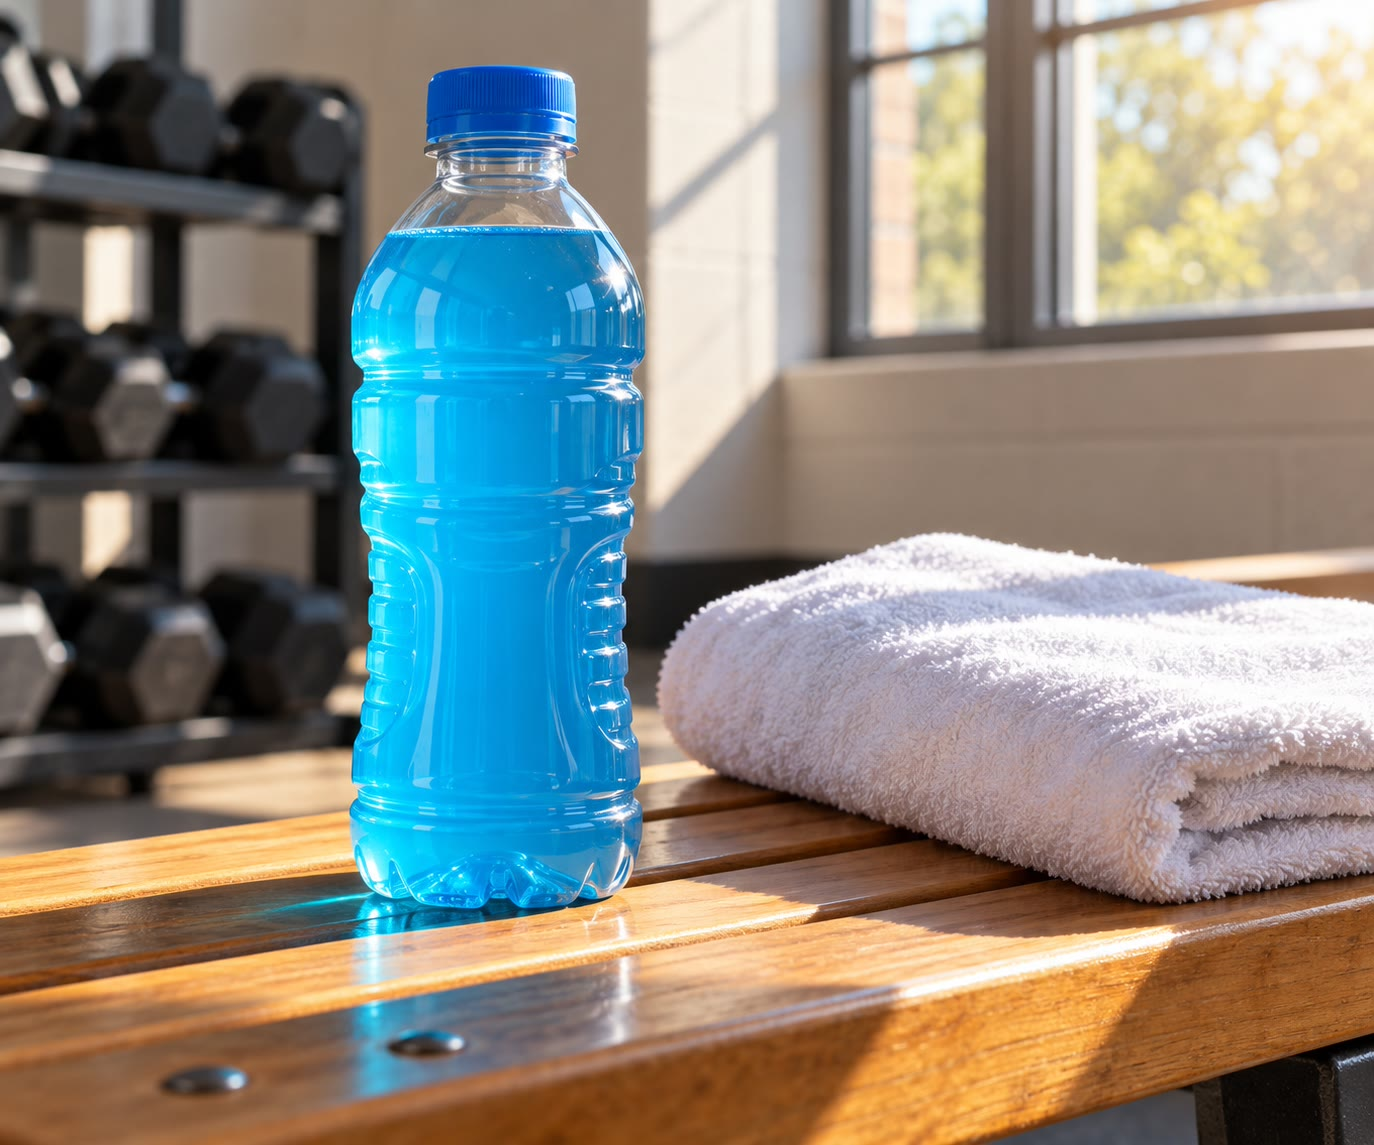
\includegraphics[width=0.5\linewidth]{images/book1/ai/g11-sports-drink.jpg}

{\small Una bebida azul: su color procede de unos pocos miligramos de
colorante por litro.}
\end{omfigure}

\section{El color de una disolución}

La luz blanca, como la luz del día, es una \omterm{def:g6:pure-substances-and-mixtures:mixture}{mezcla} de todos los colores
del arcoíris. Cada color corresponde a una longitud de onda, desde unos
\qty{400}{nm} para el violeta hasta unos \qty{750}{nm} para el rojo; el
libro de física explica qué es una longitud de onda, y aquí solo es una
etiqueta para un color. Una disolución coloreada absorbe parte de la luz
que la atraviesa, unos colores mucho más que otros; el ojo ve los
colores que pasan.

\begin{definition}[Colores complementarios]\label{def:g11:absorbance:complementary}
Dos colores son \emph{colores complementarios}\index{colores complementarios}
si al mezclarlos se obtiene luz blanca. En un círculo cromático, los
colores complementarios están enfrentados.
\end{definition}

\begin{omfigure}
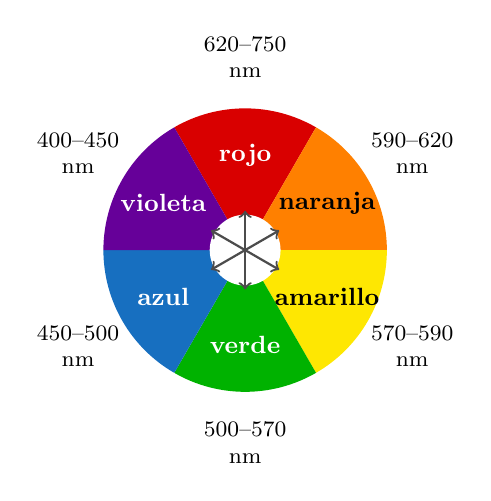
\begin{tikzpicture}[font=\small]
  \foreach \a/\c/\n/\w/\t in {90/red!85!black/rojo/{620--750}/white,
      30/orange/naranja/{590--620}/black, -30/yellow!90!orange/amarillo/{570--590}/black,
      -90/green!70!black/verde/{500--570}/white, -150/cyan!50!blue/azul/{450--500}/white,
      150/violet!80!blue/violeta/{400--450}/white} {
    \fill[\c] (0,0) -- (\a-30:1.8) arc[start angle=\a-30, end angle=\a+30,
      radius=1.8] -- cycle;
    \node[text=\t, font=\small\bfseries] at (\a:1.2) {\n};
    \node[font=\footnotesize, align=center] at (\a:2.45) {\w\\ nm};
  }
  \fill[white] (0,0) circle (0.45);
  \draw[<->, thick, black!70] (90:0.5) -- (-90:0.5);
  \draw[<->, thick, black!70] (30:0.5) -- (-150:0.5);
  \draw[<->, thick, black!70] (-30:0.5) -- (150:0.5);
\end{tikzpicture}

{\small Un círculo cromático, con longitudes de onda aproximadas. Los
\omterm{def:g11:absorbance:complementary}{colores complementarios} están enfrentados: el rojo y el verde, el
naranja y el azul, el amarillo y el violeta.}
\end{omfigure}

\begin{proposition}[El color que se ve]\label{prop:g11:absorbance:colour-seen}
Una disolución que absorbe sobre todo un color de la luz blanca se ve
del \omterm{def:g11:absorbance:complementary}{color complementario} de este.
\end{proposition}

\begin{proof}
Se admite: la luz que pasa es la luz blanca menos el color absorbido, y
el ojo ve ese resto como el \omterm{def:g11:absorbance:complementary}{color complementario}.
\end{proof}

\begin{example}[Dos colorantes alimentarios]\label{ex:g11:absorbance:dyes}
% ledger: lmax:E133, lmax:E102
El colorante azul de la bebida isotónica, llamado azul brillante
(E133), absorbe sobre todo la luz rojo anaranjada, alrededor de
\qty{629}{nm}: se ve azul. El colorante amarillo tartrazina (E102)
absorbe sobre todo la luz azul violácea, alrededor de \qty{427}{nm}: se
ve amarillo. Una bebida verde suele contener los dos.
\end{example}

\section{El espectro de absorción}

\begin{definition}[Espectro de absorción]\label{def:g11:absorbance:spectrum}
El \emph{espectro de absorción}\index{espectro de absorcion@espectro de absorción} de una
disolución es la gráfica de la luz que absorbe (su \omterm{def:g11:absorbance:absorbance}{absorbancia}, definida
en la sección siguiente) en función de la longitud de onda. La longitud
de onda a la que la absorción es máxima se escribe $\lambda_{\max}$.
\end{definition}

\begin{omfigure}
\begin{tikzpicture}
\begin{axis}[width=0.85\linewidth, height=6cm, xmin=380, xmax=750,
    ymin=0, ymax=0.95, xlabel={longitud de onda $\lambda$ (\si{nm})},
    ylabel={absorbancia $A$}, axis lines*=left, ymajorgrids,
    grid style={gray!20}, tick label style={font=\small},
    label style={font=\small}, xtick={400,450,500,550,600,650,700,750},
    ]
  % ledger: lmax:E133, abs:E133, lmax:E102, abs:E102 (band shapes synthetic)
  \addplot[very thick, cyan!60!blue] table[x=lambda, y=E133]
    {figdata/out/grade-11-absorbance-a.dat};
  \addplot[very thick, orange!85!yellow] table[x=lambda, y=E102]
    {figdata/out/grade-11-absorbance-a.dat};
  \node[font=\small, align=left, anchor=west, text=cyan!60!blue!80!black]
    at (axis cs:668,0.62) {colorante azul E133,\\ \qty{5.0}{mg/L}};
  \node[font=\small, align=left, anchor=west, text=orange!80!black]
    at (axis cs:470,0.66) {colorante amarillo E102,\\ \qty{15}{mg/L}};
  \addplot[dashed, black!50] coordinates {(629,0) (629,0.82)};
  \addplot[dashed, black!50] coordinates {(427,0) (427,0.795)};
  \node[font=\small, anchor=south] at (axis cs:629,0.83) {\qty{629}{nm}};
  \node[font=\small, anchor=south] at (axis cs:427,0.81) {\qty{427}{nm}};
\end{axis}
\end{tikzpicture}

{\small \omterm{def:g11:absorbance:spectrum}{Espectros de absorción} de los dos colorantes en agua, en una
cubeta de \qty{1}{cm} de espesor. La forma de las bandas está dibujada
con un modelo sencillo; la posición de los máximos y su altura son las
de las especificaciones de los dos colorantes.}
\end{omfigure}

\begin{remark}[Leer un espectro]\label{rem:g11:absorbance:reading}
El colorante azul no absorbe casi nada por debajo de \qty{520}{nm}: la
luz azul y la violeta pasan, y la disolución se ve azul. El colorante
amarillo no absorbe casi nada por encima de \qty{520}{nm}: la luz verde,
la amarilla, la naranja y la roja pasan, y el ojo ve amarillo. A
\qty{629}{nm} solo absorbe el colorante azul; a \qty{427}{nm}, casi
solo el amarillo.
\end{remark}

\section{La absorbancia y el espectrofotómetro}

\begin{definition}[Absorbancia]\label{def:g11:absorbance:absorbance}
La \emph{absorbancia}\index{absorbancia} $A$ de una disolución, a una
longitud de onda elegida, es el número que muestra un espectrofotómetro
que mide qué parte de la luz de esa longitud de onda absorbe la
disolución. No tiene unidad; es cero para el \omterm{def:g6:solutions-and-solubility:solute}{disolvente} puro, y es mayor
cuanta más luz absorbe la disolución.
\end{definition}

\begin{omfigure}
\begin{tikzpicture}[font=\small]
  % lamp
  \shade[ball color=yellow!40] (0,0.6) circle (0.32);
  \foreach \a in {0,45,90,135,180,225,270,315} \draw[yellow!60!orange, thick] (\a:0.4) ++(0,0.6) -- ++(\a:0.18);
  \node[anchor=north] at (0,-0.25) {lámpara};
  \draw[black!60, thick] (0.8,0.6) -- (1.75,0.6);
  % prism
  \fill[cyan!10, draw=black!60] (1.75,0.15) -- (2.55,0.15) -- (2.15,1.15) -- cycle;
  \node[anchor=north] at (2.15,-0.25) {prisma};
  \foreach \c/\d in {violet/0.35, blue/0.22, green!70!black/0.08, yellow!90!orange/-0.06,
      orange/-0.2, red/-0.34}
    \draw[\c, thick] (2.45,0.6) -- (3.45,{0.6+\d});
  % slit
  \fill[black!70] (3.5,0.92) rectangle (3.6,1.4);
  \fill[black!70] (3.5,-0.2) rectangle (3.6,0.52);
  \node[anchor=north] at (3.55,-0.25) {rendija};
  \draw[orange, very thick] (3.6,0.6) -- (4.75,0.6);
  % cuvette
  \pic (cv) at (5,0) {cuvette={0.75}{cyan!50!blue!45}};
  \node[anchor=north] at (5,-0.25) {cubeta};
  \draw[orange!60, thick] (5.3,0.6) -- (6.3,0.6);
  % detector and display
  \fill[black!15, draw=black!60] (6.3,0.2) rectangle (6.9,1.0);
  \node[anchor=north] at (6.6,-0.25) {detector};
  \draw[black!60] (6.9,0.6) -- (7.4,0.6);
  \fill[black!80, draw=black] (7.4,0.25) rectangle (9.4,0.95);
  \node[green!70!white, font=\footnotesize\ttfamily] at (8.4,0.6) {A = 0.590};
  \node[anchor=north] at (8.4,-0.25) {pantalla};
\end{tikzpicture}

{\small Principio de un espectrofotómetro. Un prisma separa la luz
blanca en sus colores; una rendija solo deja pasar una longitud de onda,
elegida por el usuario; el detector compara la luz que sale de la cubeta
con la que entra en ella, y la pantalla da la \omterm{def:g11:absorbance:absorbance}{absorbancia}.}
\end{omfigure}

\begin{remark}[De dónde sale el número]\label{rem:g11:absorbance:log}
El instrumento calcula la \omterm{def:g11:absorbance:absorbance}{absorbancia} a partir de las intensidades de la
luz que entra en la disolución y que sale de ella, con una función
matemática que se estudia en el último curso del bachillerato, el
logaritmo. Un volumen universitario da la fórmula; aquí, la \omterm{def:g11:absorbance:absorbance}{absorbancia}
es simplemente lo que marca el instrumento.
\end{remark}

\begin{inthelab}[Hacer el cero del espectrofotómetro]
La cubeta, el \omterm{def:g6:solutions-and-solubility:solute}{disolvente} y el propio instrumento absorben un poco de
luz. Antes de cualquier medida, se coloca en el instrumento una cubeta
llena del \omterm{def:g6:solutions-and-solubility:solute}{disolvente} puro, el \emph{blanco}, y se ajusta para que marque
$A = 0$ a la longitud de onda elegida. Cada lectura posterior es la
\omterm{def:g11:absorbance:absorbance}{absorbancia} del \omterm{def:g6:solutions-and-solubility:solute}{soluto} solo. Las cubetas se cogen siempre por sus caras
esmeriladas, y se limpian: una huella dactilar en una cara transparente
también absorbe luz.
\end{inthelab}

\begin{omfigure}
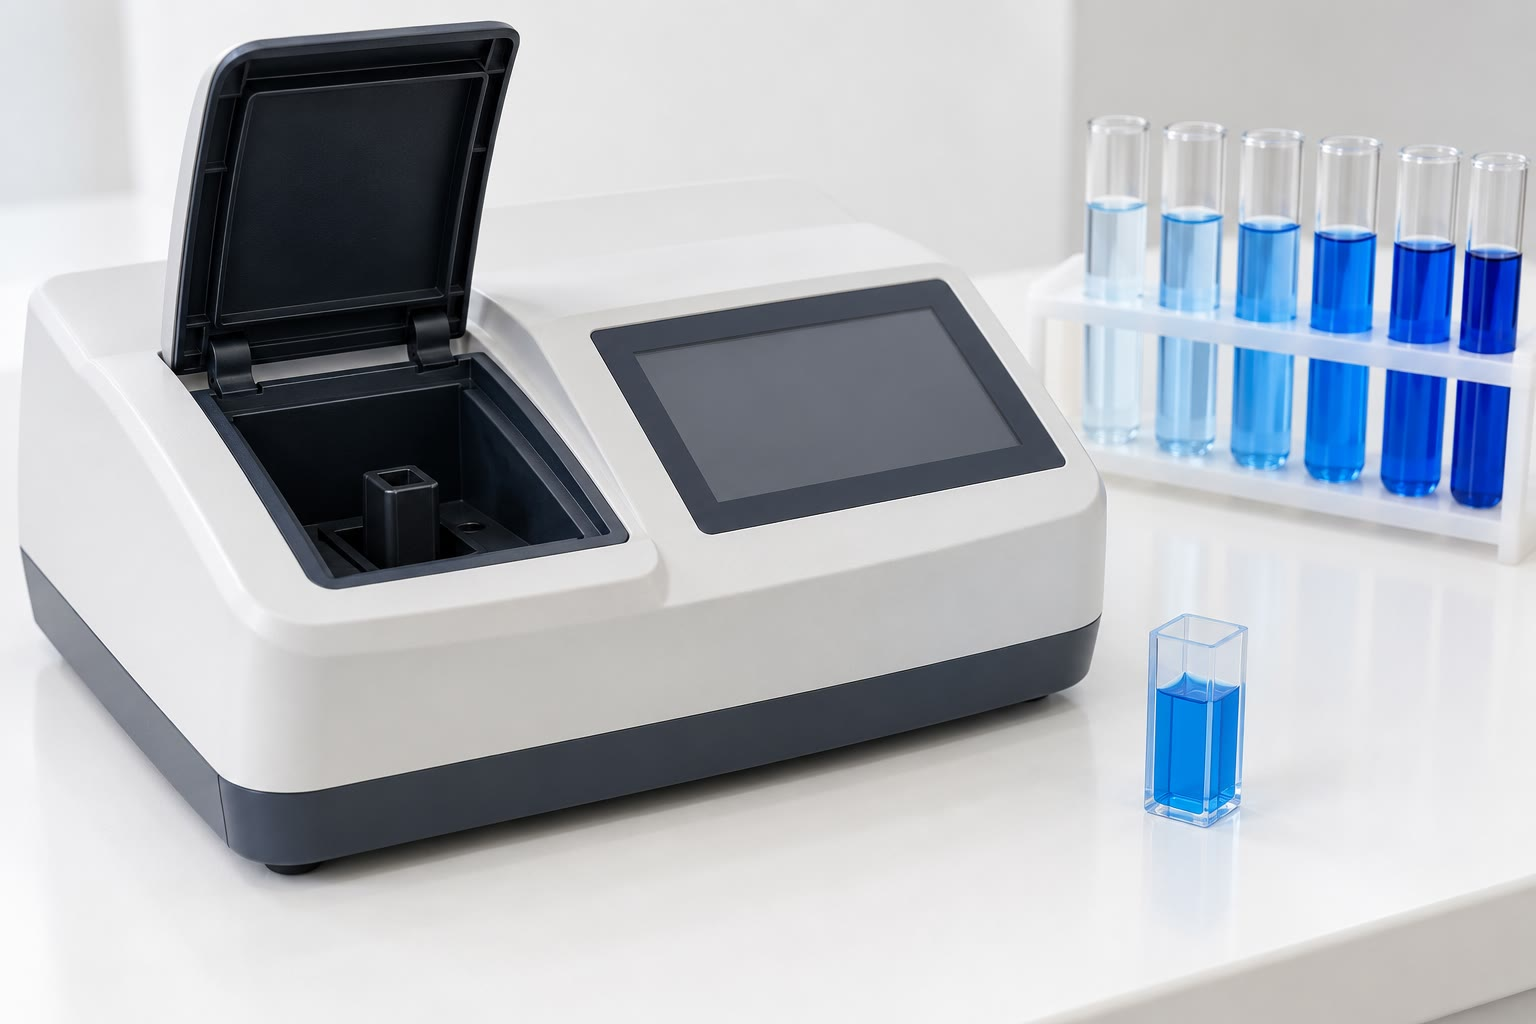
\includegraphics[width=0.5\linewidth]{images/book1/ai/g11-spectrophotometer.jpg}

{\small Un espectrofotómetro y sus cubetas cuadradas.}
\end{omfigure}

\section{La ley de Beer-Lambert}

\begin{definition}[Coeficiente de absorción molar]\label{def:g11:absorbance:epsilon}
El \emph{coeficiente de absorción molar}\index{coeficiente de absorcion molar@coeficiente de absorción molar}
$\varepsilon$ de una especie disuelta, a una longitud de onda dada, mide
con qué intensidad absorbe la luz un \omterm{def:g10:the-mole:amount}{mol} de ella; depende de la especie,
del \omterm{def:g6:solutions-and-solubility:solute}{disolvente} y de la longitud de onda, y se expresa en
\si{L/(mol.cm)}.
\end{definition}

\begin{proposition}[Ley de Beer-Lambert]\label{prop:g11:absorbance:beer-lambert}
Para una disolución diluida de una sola especie absorbente, de
\omterm{def:g10:concentration-and-dilution:molar-concentration}{concentración molar} $c$, en una cubeta de espesor $\ell$, la \omterm{def:g11:absorbance:absorbance}{absorbancia}
a una longitud de onda dada es
\[
  A = \varepsilon\, \ell\, c .
\]
La \omterm{def:g11:absorbance:absorbance}{absorbancia} es proporcional a la concentración.
\end{proposition}

\begin{proof}
Se admite aquí; se demuestra en un volumen universitario.
\end{proof}


\begin{remark}[Con una concentración en masa]\label{rem:g11:absorbance:mass}
% ledger: abs:E133, mw:E133
Como $c = C_m / M$, la ley se puede escribir también $A = a\, \ell\, C_m$,
con $a = \varepsilon / M$ en \si{L/(g.cm)}. Las especificaciones de los
colorantes alimentarios dan $a$: para el colorante azul E133 a
\qty{629}{nm}, $a =
\qty{164}{L/(g.cm)}$, y con su \omterm{def:g10:the-mole:molar-mass}{masa molar} de
\qty{792.9}{g/mol}, $\varepsilon = 164 \times 792.9 = \qty{1.30e5}{L/(mol.cm)}$.
Una disolución de solo \qty{5.0}{mg/L} de este colorante, en una cubeta
de \qty{1}{cm}, ya marca
$A = 164 \times 1 \times 0.0050 = 0.82$.
\end{remark}

\begin{remark}[Solo disoluciones diluidas]\label{rem:g11:absorbance:dilute}
La proporcionalidad solo se cumple para las disoluciones diluidas, en la
práctica para \omterm{def:g11:absorbance:absorbance}{absorbancias} inferiores a 1 o 1.5 en un instrumento
corriente. Una disolución demasiado concentrada se diluye en un factor
conocido antes de medirla.
\end{remark}

\section{Medir una concentración}

\begin{definition}[Recta de calibrado]\label{def:g11:absorbance:calibration-line}
Una \emph{recta de calibrado}\index{recta de calibrado} es la gráfica de
la \omterm{def:g11:absorbance:absorbance}{absorbancia} de una serie de \omterm{def:g10:concentration-and-dilution:standard}{disoluciones patrón} de una especie,
medidas a la misma longitud de onda y en la misma cubeta, en función de
su concentración. Cuando se cumple la ley de Beer-Lambert, es una recta
que pasa por el origen.
\end{definition}

\begin{method}[Medir una concentración con una recta de calibrado]\label{met:g11:absorbance:calibration}
\begin{enumerate}
  \item Registrar el \omterm{def:g11:absorbance:spectrum}{espectro de absorción} de la especie y elegir la
        longitud de onda $\lambda_{\max}$, donde la \omterm{def:g11:absorbance:absorbance}{absorbancia} es mayor y
        varía menos ante un pequeño error en la longitud de onda.
  \item Hacer el cero del instrumento con el blanco.
  \item Preparar \omterm{def:g10:concentration-and-dilution:standard}{disoluciones patrón} por \omterm{def:g10:concentration-and-dilution:dilution}{dilución} de una \omterm{def:g10:concentration-and-dilution:dilution}{disolución
        madre} y medir sus \omterm{def:g11:absorbance:absorbance}{absorbancias}.
  \item Representar $A$ en función de la concentración y trazar la recta
        que pasa por el origen más próxima a los puntos.
  \item Medir la desconocida, diluida si hace falta para que su
        \omterm{def:g11:absorbance:absorbance}{absorbancia} quede entre las de los patrones, y leer su
        concentración en la recta (o dividir $A$ entre la pendiente);
        multiplicar por el \omterm{def:g10:concentration-and-dilution:dilution}{factor de dilución}.
\end{enumerate}
\end{method}

\begin{omfigure}
\begin{tikzpicture}
\begin{axis}[width=0.72\linewidth, height=6cm, xmin=0, xmax=5.6,
    ymin=0, ymax=0.95, xlabel={concentración de E133 (\si{mg/L})},
    ylabel={absorbancia a \qty{629}{nm}}, axis lines*=left, ymajorgrids,
    xmajorgrids, grid style={gray!20}, tick label style={font=\small},
    label style={font=\small}]
  % ledger: abs:E133 (points synthetic: exact values + fixed offsets)
  \addplot[only marks, mark=*, mark size=2.2pt, omDef] table[x=C, y=A]
    {figdata/out/grade-11-absorbance-b.dat};
  \addplot[thick, omProp, domain=0:5.5] {0.164*x};
  \addplot[dashed, black!60] coordinates {(0,0.590) (3.6,0.590) (3.6,0)};
  \node[font=\small, anchor=south west] at (axis cs:0.1,0.6) {desconocida: $A = 0.590$};
  \node[font=\small, anchor=west] at (axis cs:3.65,0.22) {\qty{3.6}{mg/L}};
\end{axis}
\end{tikzpicture}

{\small \omterm{def:g11:absorbance:calibration-line}{Recta de calibrado} del colorante azul: cinco patrones (puntos) y
la recta que pasa por el origen, de pendiente \qty{0.164}{L/mg}. Una
desconocida que marca $A = 0.590$ tiene una concentración de $0.590 / 0.164 =
\qty{3.6}{mg/L}$.}
\end{omfigure}

\begin{example}[Los cinco patrones]\label{ex:g11:absorbance:standards}
Una \omterm{def:g10:concentration-and-dilution:dilution}{disolución madre} del colorante azul de \qty{100}{mg/L} se diluye
para obtener \qty{100.0}{mL} de cada patrón: para \qty{2.0}{mg/L}, el
\omterm{def:g10:concentration-and-dilution:dilution}{factor de dilución} es 50, así que se completan \qty{2.0}{mL} de
\omterm{def:g10:concentration-and-dilution:dilution}{disolución madre} hasta \qty{100.0}{mL}. Los cinco patrones, de 1 a
\qty{5}{mg/L}, marcan 0.168, 0.325, 0.494, 0.652 y 0.823: a unas pocas
milésimas de $0.164 \times C$, la recta de la figura.
\end{example}

\section{Ejercicios}

\begin{exercise}[$\star$]\label{exo:g11:absorbance:1}
Una disolución absorbe sobre todo la luz naranja. ¿De qué color se ve?
¿Y una disolución que absorbe sobre todo la luz violeta?
\end{exercise}

\begin{exercise}[$\star$]\label{exo:g11:absorbance:2}
Con el círculo cromático, da el color que absorbe principalmente una
disolución verde, y el intervalo de longitudes de onda que abarca ese
color.
\end{exercise}

\begin{exercise}[$\star$]\label{exo:g11:absorbance:3}
Lee en los \omterm{def:g11:absorbance:spectrum}{espectros de absorción} la longitud de onda $\lambda_{\max}$ de
cada colorante y su \omterm{def:g11:absorbance:absorbance}{absorbancia} en ese punto.
\end{exercise}

\begin{exercise}[$\star$]\label{exo:g11:absorbance:4}
Una disolución de colorante de \qty{2.0}{mg/L} marca $A = 0.30$. ¿Qué
marca una disolución del mismo colorante de \qty{6.0}{mg/L} en la misma
cubeta y a la misma longitud de onda? ¿Y una de \qty{1.0}{mg/L}?
\end{exercise}

\begin{exercise}[$\star$]\label{exo:g11:absorbance:5}
¿Qué es el blanco de un espectrofotómetro, y por qué se hace el cero
del instrumento con él?
\end{exercise}

\begin{exercise}[$\star\star$]\label{exo:g11:absorbance:6}
Con la \omterm{def:g11:absorbance:calibration-line}{recta de calibrado} del colorante azul, halla la concentración de
una disolución que marca $A = 0.41$.
\end{exercise}

\begin{exercise}[$\star\star$]\label{exo:g11:absorbance:7}
Para medir el colorante azul, ¿por qué se ajusta el espectrofotómetro a
\qty{629}{nm} y no a \qty{550}{nm}? Da dos razones.
\end{exercise}

\begin{exercise}[$\star\star$]\label{exo:g11:absorbance:8}
Una bebida sin diluir marca $A = 2.4$ a \qty{629}{nm}, un valor
demasiado alto para fiarse de él. Se diluye cinco veces y entonces marca
$A = 0.48$. Halla la concentración de colorante azul de la bebida.
\end{exercise}

\begin{exercise}[$\star\star$]\label{exo:g11:absorbance:9}
% ledger: mw:E102, abs:E102
Una disolución de tartrazina de \qty{15.0}{mg/L} marca $A = 0.795$ a
\qty{427}{nm} en una cubeta de \qty{1.00}{cm}. Calcula su absortividad
$a$ en \si{L/(g.cm)} y, después, su \omterm{def:g11:absorbance:epsilon}{coeficiente de absorción molar} (\omterm{def:g10:the-mole:molar-mass}{masa
molar} \qty{534.4}{g/mol}).
\end{exercise}

\begin{exercise}[$\star\star$]\label{exo:g11:absorbance:10}
Mira los espectros de los dos colorantes. ¿Por encima de qué longitud de
onda no absorbe casi nada el colorante amarillo? ¿Por qué se puede medir
el colorante azul a \qty{629}{nm} incluso en una bebida verde que
contiene también el colorante amarillo?
\end{exercise}

\begin{exercise}[$\star\star$]\label{exo:g11:absorbance:11}
Se mide la misma disolución en una cubeta de \qty{2.0}{cm} de espesor en
lugar de \qty{1.0}{cm}. ¿Cómo cambia su \omterm{def:g11:absorbance:absorbance}{absorbancia}? ¿Por qué?
\end{exercise}

\begin{exercise}[$\star\star\star$]\label{exo:g11:absorbance:12}
Unos patrones del colorante azul de 5, 10, 20 y \qty{40}{mg/L} marcan
0.82, 1.62, 2.30 y 2.70. Calcula $A / C$ para cada uno. ¿Qué observas?
¿Qué patrones se pueden usar para una \omterm{def:g11:absorbance:calibration-line}{recta de calibrado}, y qué habría
que hacer con una desconocida que marca $2.5$?
\end{exercise}

\begin{exercise}[$\star\star\star$]\label{exo:g11:absorbance:13}
Una bebida verde contiene el colorante azul y el amarillo. En una cubeta
de \qty{1.00}{cm} marca $A = 0.574$ a \qty{629}{nm} y $A = 0.53$ a
\qty{427}{nm}. A \qty{427}{nm} el colorante azul no absorbe casi nada, y
a \qty{629}{nm} el amarillo no absorbe nada. Halla las \omterm{def:g10:concentration-and-dilution:mass-concentration}{concentraciones
en masa} de los dos colorantes (usa $a = \qty{164}{L/(g.cm)}$ y
$a = \qty{53.0}{L/(g.cm)}$).
\end{exercise}

\begin{exercise}[$\star\star\star$]\label{exo:g11:absorbance:14}
Una alumna olvida el blanco y hace el cero del instrumento con una
cubeta vacía. Todas sus lecturas salen entonces \num{0.040} demasiado
altas. La desconocida marca $0.368$, y la alumna divide entre la
pendiente $0.164$ de la \omterm{def:g11:absorbance:calibration-line}{recta de calibrado} correcta. ¿Qué concentración
obtiene? ¿Cuál es la real? ¿En qué porcentaje se equivoca?
\end{exercise}

\begin{exercise}[$\star\star\star$]\label{exo:g11:absorbance:15}
% ledger: adi:E102
La ingesta diaria admisible de tartrazina es de \qty{10}{mg} por
kilogramo de masa corporal. Una bebida contiene \qty{20}{mg/L}. ¿Qué
volumen de bebida llevaría a un adulto de \qty{60}{kg} hasta esa ingesta
en un día? ¿Es un riesgo realista?
\end{exercise}

\section{Problema: El azul de una bebida isotónica}


\begin{problem}[{Problema de fin de semana --- ¿cuántas botellas de una
bebida isotónica azul tendría que beber un niño para alcanzar el límite
diario seguro de su colorante?}]
\label{pb:g11:absorbance:1}
% ledger: lmax:E133, abs:E133, mw:E133, adi:E133
Un laboratorio de alimentos controla el colorante azul E133 de una
bebida isotónica que se vende en botellas de \qty{500}{mL}. Las
especificaciones del colorante dan su \omterm{def:g10:the-mole:molar-mass}{masa molar}, \qty{792.9}{g/mol}, y
su ingesta diaria admisible: \qty{6}{mg} por kilogramo de masa corporal
y por día, una cantidad que se puede tomar todos los días durante toda
la vida sin riesgo apreciable.

\medskip
\noindent\textbf{Parte I --- Color y espectro.}
\begin{enumerate}
  \item La bebida se ve azul. Con el círculo cromático, ¿qué color de
        luz absorbe más?
  \item Lee la longitud de onda $\lambda_{\max}$ del colorante en su
        espectro.
  \item ¿Por qué la \omterm{def:g11:absorbance:absorbance}{absorbancia} del colorante es casi nula a
        \qty{450}{nm}? ¿Concuerda esto con su color?
  \item ¿A qué longitud de onda hay que hacer las medidas?
\end{enumerate}

\medskip
\noindent\textbf{Parte II --- La \omterm{def:g11:absorbance:calibration-line}{recta de calibrado}.}
\begin{enumerate}[resume]
  \item Se \omterm{def:g2:mixing-and-dissolving:dissolve}{disuelven} \qty{50.0}{mg} de colorante puro para obtener
        \qty{500.0}{mL} de \omterm{def:g10:concentration-and-dilution:dilution}{disolución madre}. Calcula su \omterm{def:g10:concentration-and-dilution:mass-concentration}{concentración en
        masa} en \si{mg/L}.
  \item Se preparan patrones de 1.0, 2.0, 3.0, 4.0 y \qty{5.0}{mg/L}, de
        \qty{100.0}{mL} cada uno. ¿Qué volumen de \omterm{def:g10:concentration-and-dilution:dilution}{disolución madre} hace
        falta para el patrón de \qty{3.0}{mg/L}? ¿Con qué material de
        vidrio?
  \item Los patrones marcan 0.168, 0.325, 0.494, 0.652 y 0.823. Calcula
        $A / C$ para cada uno y muestra que los puntos están cerca de
        una recta que pasa por el origen, de pendiente de unos
        \qty{0.164}{L/mg}.
  \item ¿Por qué tiene que pasar la recta por el origen?
  \item Deduce la absortividad $a$ del colorante en \si{L/(g.cm)}
        (cubeta de \qty{1.00}{cm}) y, después, su \omterm{def:g11:absorbance:epsilon}{coeficiente de
        absorción molar}.
\end{enumerate}

\medskip
\noindent\textbf{Parte III --- La bebida.}
\begin{enumerate}[resume]
  \item Se completan \qty{25.0}{mL} de bebida hasta \qty{50.0}{mL} con
        agua. ¿Cuál es el \omterm{def:g10:concentration-and-dilution:dilution}{factor de dilución}?
  \item La bebida diluida marca $A = 0.590$. Halla su concentración de
        colorante.
  \item Deduce la concentración de colorante de la propia bebida.
  \item ¿Qué marcaría la bebida sin diluir? ¿Por qué se diluyó?
  \item Calcula la masa de colorante de una botella.
  \item Calcula la cantidad de colorante, en \omterm{def:g10:the-mole:amount}{moles}, de una botella.
\end{enumerate}

\medskip
\noindent\textbf{Parte IV --- La ingesta diaria admisible.}
\begin{enumerate}[resume]
  \item ¿Qué masa de colorante puede tomar cada día un niño de
        \qty{30}{kg}?
  \item ¿Cuántas botellas tendría que beber el niño en un día para
        alcanzarla?
  \item ¿Qué volumen de bebida es eso? Coméntalo.
  \item La misma pregunta para un adulto de \qty{70}{kg}.
  \item Da la respuesta final: ¿cuántas botellas de \qty{500}{mL}
        tendría que beber en un día un niño de \qty{30}{kg} para
        alcanzar la ingesta diaria admisible del colorante?
\end{enumerate}
\end{problem}
